

\tikzset{every picture/.style={line width=0.75pt}} %set default line width to 0.75pt        

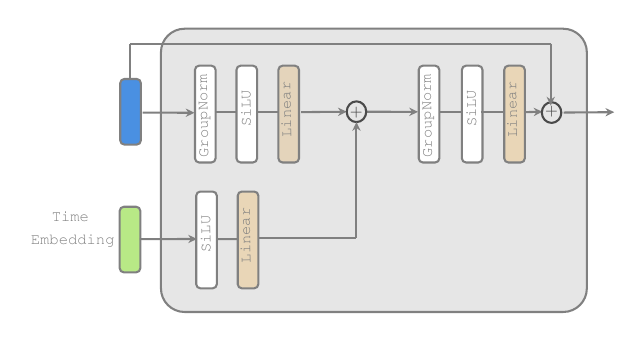
\begin{tikzpicture}[x=0.75pt,y=0.75pt,yscale=-1,xscale=1,scale=0.8]
%uncomment if require: \path (0,199); %set diagram left start at 0, and has height of 199

%Rounded Rect [id:dp23369966317189172] 
\draw  [color={rgb, 255:red, 128; green, 128; blue, 128 }  ,draw opacity=1 ][fill={rgb, 255:red, 245; green, 166; blue, 35 }  ,fill opacity=0.24 ] (361.85,35.48) .. controls (361.85,34.11) and (362.96,33) .. (364.33,33) -- (371.77,33) .. controls (373.14,33) and (374.25,34.11) .. (374.25,35.48) -- (374.25,88.8) .. controls (374.25,90.17) and (373.14,91.28) .. (371.77,91.28) -- (364.33,91.28) .. controls (362.96,91.28) and (361.85,90.17) .. (361.85,88.8) -- cycle ;

%Rounded Rect [id:dp47916639498650393] 
\draw  [color={rgb, 255:red, 128; green, 128; blue, 128 }  ,draw opacity=1 ][fill={rgb, 255:red, 184; green, 233; blue, 134 }  ,fill opacity=1 ] (266.27,120.43) .. controls (266.27,119.06) and (267.38,117.95) .. (268.75,117.95) -- (276.19,117.95) .. controls (277.56,117.95) and (278.67,119.06) .. (278.67,120.43) -- (278.67,154.97) .. controls (278.67,156.34) and (277.56,157.45) .. (276.19,157.45) -- (268.75,157.45) .. controls (267.38,157.45) and (266.27,156.34) .. (266.27,154.97) -- cycle ;
%Rounded Rect [id:dp8420620309987483] 
\draw  [color={rgb, 255:red, 128; green, 128; blue, 128 }  ,draw opacity=1 ][fill={rgb, 255:red, 74; green, 144; blue, 226 }  ,fill opacity=1 ] (266.6,43.48) .. controls (266.6,42.11) and (267.71,41) .. (269.08,41) -- (276.52,41) .. controls (277.89,41) and (279,42.11) .. (279,43.48) -- (279,78.02) .. controls (279,79.39) and (277.89,80.5) .. (276.52,80.5) -- (269.08,80.5) .. controls (267.71,80.5) and (266.6,79.39) .. (266.6,78.02) -- cycle ;
%Rounded Rect [id:dp4961571836770784] 
\draw  [color={rgb, 255:red, 128; green, 128; blue, 128 }  ,draw opacity=1 ][fill={rgb, 255:red, 128; green, 128; blue, 128 }  ,fill opacity=0.2 ] (291.1,24.97) .. controls (291.1,17.1) and (297.48,10.72) .. (305.35,10.72) -- (533.35,10.72) .. controls (541.22,10.72) and (547.6,17.1) .. (547.6,24.97) -- (547.6,167.07) .. controls (547.6,174.94) and (541.22,181.32) .. (533.35,181.32) -- (305.35,181.32) .. controls (297.48,181.32) and (291.1,174.94) .. (291.1,167.07) -- cycle ;
%Rounded Rect [id:dp43011173971404815] 
\draw  [color={rgb, 255:red, 128; green, 128; blue, 128 }  ,draw opacity=1 ][fill={rgb, 255:red, 245; green, 166; blue, 35 }  ,fill opacity=0.24 ] (337.35,111.27) .. controls (337.35,109.9) and (338.46,108.79) .. (339.83,108.79) -- (347.27,108.79) .. controls (348.64,108.79) and (349.75,109.9) .. (349.75,111.27) -- (349.75,164.59) .. controls (349.75,165.96) and (348.64,167.07) .. (347.27,167.07) -- (339.83,167.07) .. controls (338.46,167.07) and (337.35,165.96) .. (337.35,164.59) -- cycle ;

%Rounded Rect [id:dp7638773198152089] 
\draw  [color={rgb, 255:red, 128; green, 128; blue, 128 }  ,draw opacity=1 ][fill={rgb, 255:red, 255; green, 255; blue, 255 }  ,fill opacity=1 ] (311.6,35.48) .. controls (311.6,34.11) and (312.71,33) .. (314.08,33) -- (321.52,33) .. controls (322.89,33) and (324,34.11) .. (324,35.48) -- (324,88.8) .. controls (324,90.17) and (322.89,91.28) .. (321.52,91.28) -- (314.08,91.28) .. controls (312.71,91.28) and (311.6,90.17) .. (311.6,88.8) -- cycle ;
%Rounded Rect [id:dp43295255482017425] 
\draw  [color={rgb, 255:red, 128; green, 128; blue, 128 }  ,draw opacity=1 ][fill={rgb, 255:red, 255; green, 255; blue, 255 }  ,fill opacity=1 ] (312.35,111.27) .. controls (312.35,109.9) and (313.46,108.79) .. (314.83,108.79) -- (322.27,108.79) .. controls (323.64,108.79) and (324.75,109.9) .. (324.75,111.27) -- (324.75,164.59) .. controls (324.75,165.96) and (323.64,167.07) .. (322.27,167.07) -- (314.83,167.07) .. controls (313.46,167.07) and (312.35,165.96) .. (312.35,164.59) -- cycle ;

%Straight Lines [id:da6300259185680861] 
\draw [color={rgb, 255:red, 128; green, 128; blue, 128 }  ,draw opacity=1 ]   (375.56,60.96) -- (399.98,60.74) ;
\draw [shift={(402.98,60.71)}, rotate = 179.48] [fill={rgb, 255:red, 128; green, 128; blue, 128 }  ,fill opacity=1 ][line width=0.08]  [draw opacity=0] (5.36,-2.57) -- (0,0) -- (5.36,2.57) -- (3.56,0) -- cycle    ;
%Straight Lines [id:da9054213973773921] 
\draw [color={rgb, 255:red, 128; green, 128; blue, 128 }  ,draw opacity=1 ]   (280.1,61.25) -- (308.3,61.33) ;
\draw [shift={(311.3,61.33)}, rotate = 180.15] [fill={rgb, 255:red, 128; green, 128; blue, 128 }  ,fill opacity=1 ][line width=0.08]  [draw opacity=0] (5.36,-2.57) -- (0,0) -- (5.36,2.57) -- (3.56,0) -- cycle    ;
%Rounded Rect [id:dp8010430405839879] 
\draw  [color={rgb, 255:red, 128; green, 128; blue, 128 }  ,draw opacity=1 ][fill={rgb, 255:red, 255; green, 255; blue, 255 }  ,fill opacity=1 ] (336.6,35.48) .. controls (336.6,34.11) and (337.71,33) .. (339.08,33) -- (346.52,33) .. controls (347.89,33) and (349,34.11) .. (349,35.48) -- (349,88.8) .. controls (349,90.17) and (347.89,91.28) .. (346.52,91.28) -- (339.08,91.28) .. controls (337.71,91.28) and (336.6,90.17) .. (336.6,88.8) -- cycle ;

%Rounded Rect [id:dp5422664842896772] 
\draw  [color={rgb, 255:red, 128; green, 128; blue, 128 }  ,draw opacity=1 ][fill={rgb, 255:red, 245; green, 166; blue, 35 }  ,fill opacity=0.24 ] (497.85,35.48) .. controls (497.85,34.11) and (498.96,33) .. (500.33,33) -- (507.77,33) .. controls (509.14,33) and (510.25,34.11) .. (510.25,35.48) -- (510.25,88.8) .. controls (510.25,90.17) and (509.14,91.28) .. (507.77,91.28) -- (500.33,91.28) .. controls (498.96,91.28) and (497.85,90.17) .. (497.85,88.8) -- cycle ;

%Rounded Rect [id:dp025869468698855425] 
\draw  [color={rgb, 255:red, 128; green, 128; blue, 128 }  ,draw opacity=1 ][fill={rgb, 255:red, 255; green, 255; blue, 255 }  ,fill opacity=1 ] (446.35,35.48) .. controls (446.35,34.11) and (447.46,33) .. (448.83,33) -- (456.27,33) .. controls (457.64,33) and (458.75,34.11) .. (458.75,35.48) -- (458.75,88.8) .. controls (458.75,90.17) and (457.64,91.28) .. (456.27,91.28) -- (448.83,91.28) .. controls (447.46,91.28) and (446.35,90.17) .. (446.35,88.8) -- cycle ;
%Straight Lines [id:da2571975167320093] 
\draw [color={rgb, 255:red, 128; green, 128; blue, 128 }  ,draw opacity=1 ]   (510.31,60.96) -- (517.85,60.79) ;
\draw [shift={(520.85,60.72)}, rotate = 178.72] [fill={rgb, 255:red, 128; green, 128; blue, 128 }  ,fill opacity=1 ][line width=0.08]  [draw opacity=0] (5.36,-2.57) -- (0,0) -- (5.36,2.57) -- (3.56,0) -- cycle    ;
%Straight Lines [id:da10850616281834768] 
\draw [color={rgb, 255:red, 128; green, 128; blue, 128 }  ,draw opacity=1 ]   (414.73,60.71) -- (442.93,60.79) ;
\draw [shift={(445.93,60.79)}, rotate = 180.15] [fill={rgb, 255:red, 128; green, 128; blue, 128 }  ,fill opacity=1 ][line width=0.08]  [draw opacity=0] (5.36,-2.57) -- (0,0) -- (5.36,2.57) -- (3.56,0) -- cycle    ;
%Rounded Rect [id:dp07698438276657904] 
\draw  [color={rgb, 255:red, 128; green, 128; blue, 128 }  ,draw opacity=1 ][fill={rgb, 255:red, 255; green, 255; blue, 255 }  ,fill opacity=1 ] (472.35,35.48) .. controls (472.35,34.11) and (473.46,33) .. (474.83,33) -- (482.27,33) .. controls (483.64,33) and (484.75,34.11) .. (484.75,35.48) -- (484.75,88.8) .. controls (484.75,90.17) and (483.64,91.28) .. (482.27,91.28) -- (474.83,91.28) .. controls (473.46,91.28) and (472.35,90.17) .. (472.35,88.8) -- cycle ;

%Straight Lines [id:da9761794640373043] 
\draw [color={rgb, 255:red, 128; green, 128; blue, 128 }  ,draw opacity=1 ]   (323.6,60.96) -- (336.85,60.96) ;
%Straight Lines [id:da24544653033028951] 
\draw [color={rgb, 255:red, 128; green, 128; blue, 128 }  ,draw opacity=1 ]   (348.6,60.96) -- (361.85,60.96) ;
%Straight Lines [id:da18959005924368233] 
\draw [color={rgb, 255:red, 128; green, 128; blue, 128 }  ,draw opacity=1 ]   (278.35,137.48) -- (309.8,137.35) ;
\draw [shift={(312.8,137.33)}, rotate = 179.76] [fill={rgb, 255:red, 128; green, 128; blue, 128 }  ,fill opacity=1 ][line width=0.08]  [draw opacity=0] (5.36,-2.57) -- (0,0) -- (5.36,2.57) -- (3.56,0) -- cycle    ;
%Straight Lines [id:da04979064189987126] 
\draw [color={rgb, 255:red, 128; green, 128; blue, 128 }  ,draw opacity=1 ]   (458.85,60.96) -- (472.1,60.96) ;
%Straight Lines [id:da6174852451143575] 
\draw [color={rgb, 255:red, 128; green, 128; blue, 128 }  ,draw opacity=1 ]   (483.85,60.96) -- (497.1,60.96) ;
%Shape: Ellipse [id:dp17934011100408243] 
\draw  [color={rgb, 255:red, 74; green, 74; blue, 74 }  ,draw opacity=1 ] (402.98,60.71) .. controls (402.98,57.27) and (405.61,54.47) .. (408.85,54.47) .. controls (412.1,54.47) and (414.73,57.27) .. (414.73,60.71) .. controls (414.73,64.16) and (412.1,66.95) .. (408.85,66.95) .. controls (405.61,66.95) and (402.98,64.16) .. (402.98,60.71) -- cycle ;
%Straight Lines [id:da46584024123365464] 
\draw [color={rgb, 255:red, 128; green, 128; blue, 128 }  ,draw opacity=1 ]   (325.1,137.46) -- (336.85,137.47) ;
%Straight Lines [id:da8918614298059904] 
\draw [color={rgb, 255:red, 128; green, 128; blue, 128 }  ,draw opacity=1 ]   (349.85,137) -- (408.85,137) ;
%Straight Lines [id:da12409138747216075] 
\draw [color={rgb, 255:red, 128; green, 128; blue, 128 }  ,draw opacity=1 ]   (408.85,137) -- (408.85,69.95) ;
\draw [shift={(408.85,66.95)}, rotate = 90] [fill={rgb, 255:red, 128; green, 128; blue, 128 }  ,fill opacity=1 ][line width=0.08]  [draw opacity=0] (5.36,-2.57) -- (0,0) -- (5.36,2.57) -- (3.56,0) -- cycle    ;
%Straight Lines [id:da9995181107635376] 
\draw [color={rgb, 255:red, 128; green, 128; blue, 128 }  ,draw opacity=1 ]   (272.47,19.75) -- (525.85,19.75) ;
%Shape: Ellipse [id:dp25472045356952755] 
\draw  [color={rgb, 255:red, 74; green, 74; blue, 74 }  ,draw opacity=1 ] (520.48,61.21) .. controls (520.48,57.77) and (523.11,54.97) .. (526.35,54.97) .. controls (529.6,54.97) and (532.23,57.77) .. (532.23,61.21) .. controls (532.23,64.66) and (529.6,67.45) .. (526.35,67.45) .. controls (523.11,67.45) and (520.48,64.66) .. (520.48,61.21) -- cycle ;
%Straight Lines [id:da5995871556506267] 
\draw [color={rgb, 255:red, 128; green, 128; blue, 128 }  ,draw opacity=1 ]   (533.56,61.21) -- (561.1,61) ;
\draw [shift={(564.1,60.97)}, rotate = 179.56] [fill={rgb, 255:red, 128; green, 128; blue, 128 }  ,fill opacity=1 ][line width=0.08]  [draw opacity=0] (5.36,-2.57) -- (0,0) -- (5.36,2.57) -- (3.56,0) -- cycle    ;
%Straight Lines [id:da18808498976213528] 
\draw [color={rgb, 255:red, 128; green, 128; blue, 128 }  ,draw opacity=1 ]   (272.47,40.72) -- (272.47,19.75) ;
%Straight Lines [id:da3136929839120528] 
\draw [color={rgb, 255:red, 128; green, 128; blue, 128 }  ,draw opacity=1 ]   (525.85,19.75) -- (525.85,53.97) ;
\draw [shift={(525.85,56.97)}, rotate = 270] [fill={rgb, 255:red, 128; green, 128; blue, 128 }  ,fill opacity=1 ][line width=0.08]  [draw opacity=0] (5.36,-2.57) -- (0,0) -- (5.36,2.57) -- (3.56,0) -- cycle    ;

% Text Node
\draw (362.11,77.64) node [anchor=north west][inner sep=0.75pt]  [font=\scriptsize,rotate=-269.05,xscale=0.7,yscale=0.7] [align=left] {{\fontfamily{pcr}\selectfont \textcolor[rgb]{0.5,0.5,0.5}{{\footnotesize Linear}}}};
% Text Node
\draw (337.61,153.42) node [anchor=north west][inner sep=0.75pt]  [font=\scriptsize,rotate=-269.05,xscale=0.7,yscale=0.7] [align=left] {{\fontfamily{pcr}\selectfont \textcolor[rgb]{0.5,0.5,0.5}{{\footnotesize Linear}}}};
% Text Node
\draw (211.47,119.06) node [anchor=north west][inner sep=0.75pt]  [xscale=0.7,yscale=0.7] [align=left] {\begin{minipage}[lt]{40.83pt}\setlength\topsep{0pt}
\begin{center}
\textcolor[rgb]{0.5,0.5,0.5}{{\footnotesize {\fontfamily{pcr}\selectfont Time}}}\\{\fontfamily{pcr}\selectfont \textcolor[rgb]{0.5,0.5,0.5}{{\footnotesize Embedding}}}
\end{center}

\end{minipage}};
% Text Node
\draw (313.61,147.08) node [anchor=north west][inner sep=0.75pt]  [font=\scriptsize,rotate=-269.05,xscale=0.7,yscale=0.7] [align=left] {{\fontfamily{pcr}\selectfont \textcolor[rgb]{0.5,0.5,0.5}{{\footnotesize SiLU}}}};
% Text Node
\draw (337.86,71.29) node [anchor=north west][inner sep=0.75pt]  [font=\scriptsize,rotate=-269.05,xscale=0.7,yscale=0.7] [align=left] {{\fontfamily{pcr}\selectfont \textcolor[rgb]{0.5,0.5,0.5}{{\footnotesize SiLU}}}};
% Text Node
\draw (473.61,71.29) node [anchor=north west][inner sep=0.75pt]  [font=\scriptsize,rotate=-269.05,xscale=0.7,yscale=0.7] [align=left] {{\fontfamily{pcr}\selectfont \textcolor[rgb]{0.5,0.5,0.5}{{\footnotesize SiLU}}}};
% Text Node
\draw (498.11,77.64) node [anchor=north west][inner sep=0.75pt]  [font=\scriptsize,rotate=-269.05,xscale=0.7,yscale=0.7] [align=left] {{\fontfamily{pcr}\selectfont \textcolor[rgb]{0.5,0.5,0.5}{{\footnotesize Linear}}}};
% Text Node
\draw (403.6,56.72) node [anchor=north west][inner sep=0.75pt]  [font=\footnotesize,color={rgb, 255:red, 74; green, 74; blue, 74 }  ,opacity=1 ,xscale=0.7,yscale=0.7]  {$\mathnormal{+}$};
% Text Node
\draw (312.86,89.64) node [anchor=north west][inner sep=0.75pt]  [font=\scriptsize,rotate=-269.05,xscale=0.7,yscale=0.7] [align=left] {{\fontfamily{pcr}\selectfont \textcolor[rgb]{0.5,0.5,0.5}{{\footnotesize GroupNorm}}}};
% Text Node
\draw (447.61,89.64) node [anchor=north west][inner sep=0.75pt]  [font=\scriptsize,rotate=-269.05,xscale=0.7,yscale=0.7] [align=left] {{\fontfamily{pcr}\selectfont \textcolor[rgb]{0.5,0.5,0.5}{{\footnotesize GroupNorm}}}};
% Text Node
\draw (521.1,56.22) node [anchor=north west][inner sep=0.75pt]  [font=\footnotesize,color={rgb, 255:red, 74; green, 74; blue, 74 }  ,opacity=1 ,xscale=0.7,yscale=0.7]  {$\mathnormal{+}$};


\end{tikzpicture}